\documentclass[final]{beamer}
\usepackage[T1]{fontenc}
\usepackage{lmodern}
\usepackage[size=custom,width=120,height=72,scale=1.0]{beamerposter}
\usetheme{gemini}
\usecolortheme{gemini}
\usepackage{graphicx}
\usepackage{booktabs}
\usepackage{tikz}
\usepackage{pgfplots}
\usepackage{csquotes}
\usepackage[
backend=biber,
style=numeric,
citestyle=numeric
]{biblatex}
\addbibresource{biblio.bib}

\usepackage[font=small,labelfont=bf]{caption} 

\newcommand{\compresslist}{
  \setlength{\itemsep}{1pt}
  \setlength{\parskip}{0pt}
  \setlength{\parsep}{0pt}}

\newcommand{\bfSigma}{\mbox{\boldmath$\Sigma$}}
\newcommand{\bfLambda}{\mbox{\boldmath$\Lambda$}}
\DeclareMathOperator*{\argmax}{\arg\!\max}
% ====================
% Lengths
% ====================

% If you have N columns, choose \sepwidth and \colwidth such that
% (N+1)*\sepwidth + N*\colwidth = \paperwidth
\newlength{\sepwidth}
\newlength{\colwidth}
\setlength{\sepwidth}{0.025\paperwidth}
\setlength{\colwidth}{0.3\paperwidth}
\newcommand{\separatorcolumn}{\begin{column}{\sepwidth}\end{column}}

% ====================
% Title
% ====================
\title{Text Sequence Generation and Classification, model or inference}
\author{Jimmy Leroux, Nicolas Laliberté, Frédéric Boileau}

\institute[]{Départment d'Informatique et de Recherche Opérationnelle -
Université de Montréal}

% ====================
% Body
% ====================

\begin{document}
\begin{frame}[t]
\begin{columns}[t]
\separatorcolumn

\begin{column}{\colwidth}

\begin{block}{Introduction}
\begin{itemize}
\item Hidden Markov Models used to be the go-to probabilistic tool to model 
sequential data; the Markov assumption however proves to often be unreasonably
strong. Adding links to form higher order chains is not a scalable solution as
the computationnal complexity grows exponentially in the order of the chain.

\item Recurrent Neural Networks (RNN) constitute a family of neural network
architectures specialized to process sequential data which can forfeit
Markovian assumptions while remaining tractable.


\item RNN enable to track longer range dependencies while staying tractable by
    leveraging the simple idea of sharing parameters across the model
    \cite{deeplearning}. Concretely this means adding loops to the hidden units
    of the neural network.

\item RNNs have been used in diverse domains for
  generating sequences such as music and text \cite{gravesGenerating}. 

\item Despite the aforementionned features, RNN suffer from the fact 
that the influence of some input the hidden layer either decays or blows up
exponentially in time, a phenomenon reffered to in the literature as the
\textit{vanishing gradient problem}.
\end{itemize}
The cost of abandonning probabilistic models such as the HMM in favor of neural
networks is the loss of a fully probabilistic interpretation. There has
recently been an increased interest into finding reasonable probabilistic
interpretaions to RNNs, see for example \cite{finnish}. On the other hand the
very existence of some monolithic notion of ``interpretability'' has been
recently questionned, see \cite{mythos} for a philosophical overview and the
interesting blog post by Jacob Andreas on the blur between a model and an
inference procedure in RNNs.\cite{monference}
\end{block}

\begin{block}{RNN} 
\begin{center}
    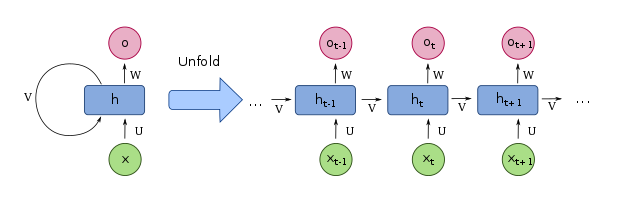
\includegraphics[width = 0.9\linewidth]{RNN.png}
\end{center}
\begin{equation*}
    h_t = \sigma(U x_t + V h_{(t-1)} + b_h)\text{,}
    \qquad o_t = \text{softmax}(W h_t + b_o)
\end{equation*}
\small{Where $ U$, $V$ and $W$ are weights matrix and the vectors $b$ are bias
parameters.}\\

\normalsize
Consider the gradient of $o_{t + \delta}$ with respect to $h_t$.\\
Applying the chain rule according to the graph above we get:

\begin{equation*}
  \nabla_{h_t} o_{t + \delta} = \left( \prod_{k = t+1}^{t+\delta} V^T
  \text{diag}(1 - h^2_k) \right)\nabla_{h_{t + \delta}}o_{t + \delta}.
\end{equation*}

Thus, as $\delta$ grows, the gradient grows exponentially with $V$. If $V$ is
small or large than the gradient will either vanish or explode. A myriad
of solutions exist such as regularization through weight noise, the LSTM
architecture tries to tackle this issue on a higher level than regularization.
\end{block}
\end{column}
\separatorcolumn

\begin{column}{\colwidth}

\begin{block}{LSTM: architecture and its application to sequence generation}

The LSTM model has been introduced primarily to solve the vanishing and
exploding gradients problem. This model is a RNN in which we replaced every
hidden nodes by a \textit{memory cell}.  \begin{center}
    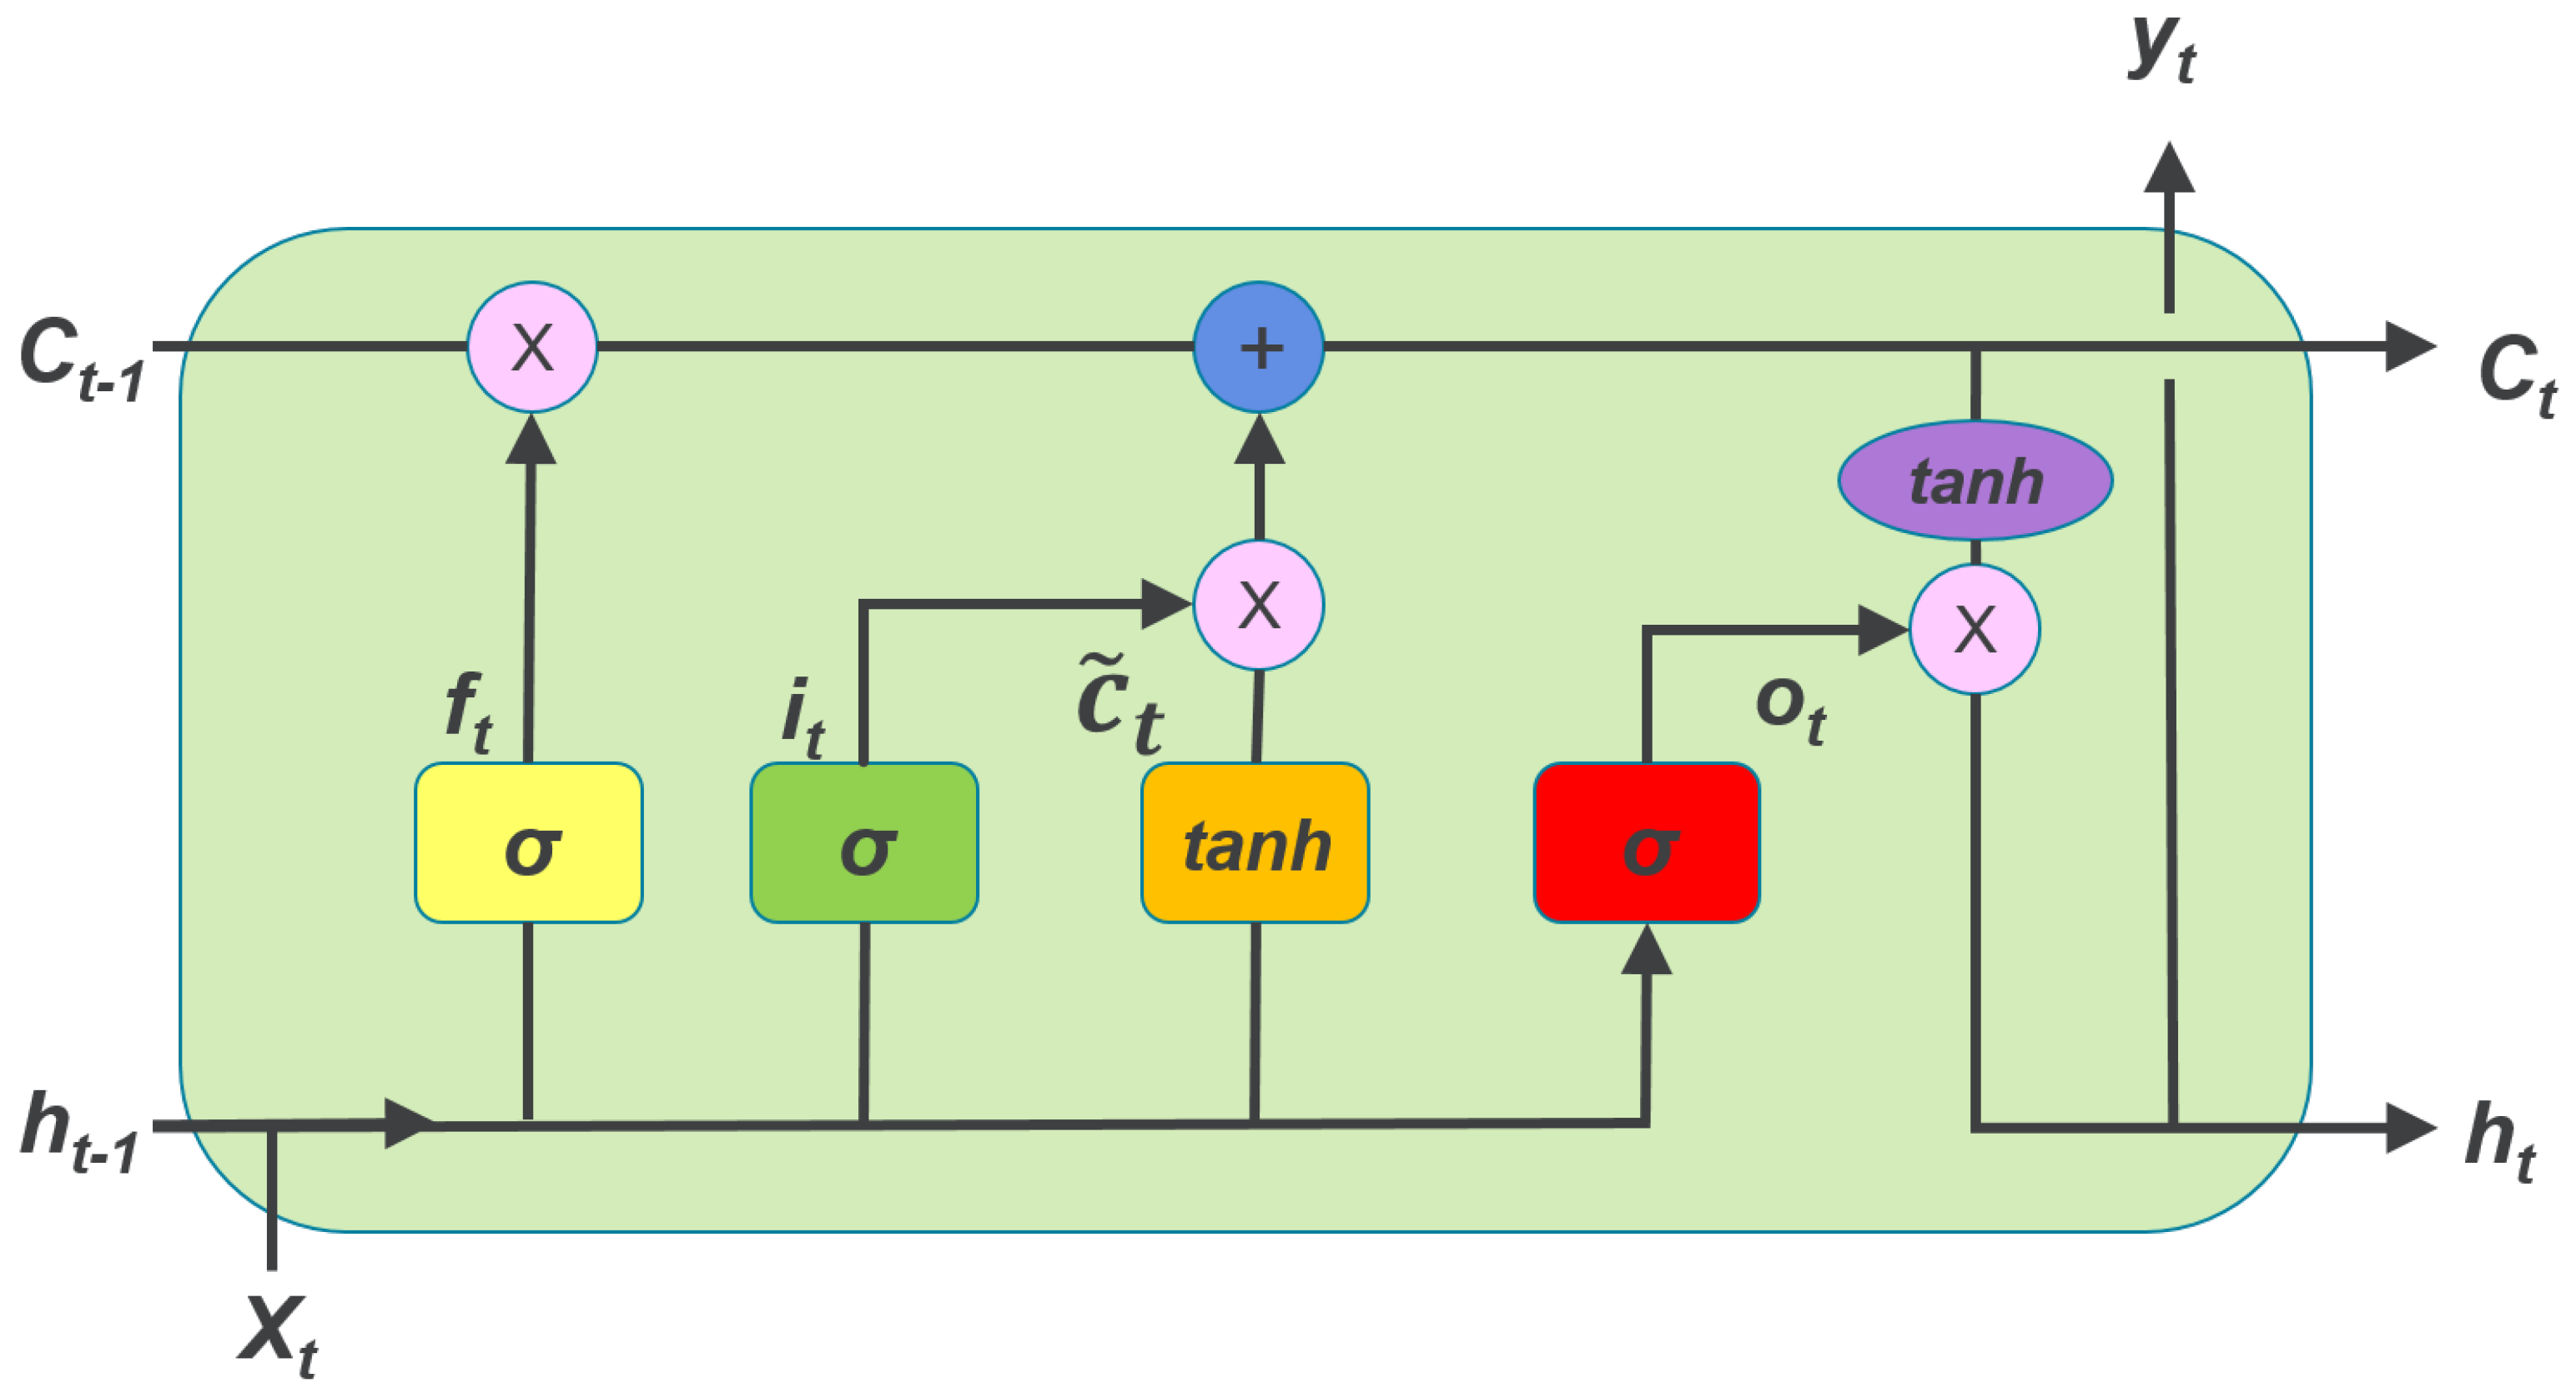
\includegraphics[width = 0.7\linewidth]{lstm.png}
\end{center}

Intuitively, RNN have \textit{long-term memory} in the form of matrix weights,
they change during the training encoding general knowledge about the data. RNN
also have \textit{short-term memory} in the form of activation passing from
each node to successive ones. The memory cell introduced in the LSTM model
provides storage for those memories. We now describe components of the cell
following.\cite{review}

\begin{center}
    \begin{itemize}
    \item Gates ($f_t, i_t, o_t$): They are sigmoidal units that takes
      activation from the input $x_t$ and the output of the hidden layer from
      previous state $h_{t-1}$. Note that $f_t$ multiply the value of the
      previous cell $c_{t-1}$. The term \textit{gate} stands for the literal
      meaning in the sense that if $f_{t}$ is close to $0$, then the gate is
      \textit{closed} and the flow from the previous cell is cut off. If $f_t$
      is closed to $1$ then all flow is passed through. The output to the
      hidden layer is $h_t = o_t \odot \tanh(c_t)$ where $\odot$ denote the
      pointwise multiplication.
    \item Cell state ($c_t = f_t \odot c_{t-1} + i_t \odot \tilde{c}_t$): Cell
    state maintains information on the input. Also refered as the internal state,
    $c_t$ has a self-connected edges with a fixed unit weight. This constant
    weight implies that the error can flow across time without vanishing or
    exploding. 
\end{itemize}
\end{center}

\end{block}

\begin{block}{Our implementation}
For the implementation section of this project, we gathered text data that we
found around the internet to train a sequence classifier and generate text
sequences. The training of the classifier consist of identifying from which
corpus between Harry Potter, Lord of the rings, some random quotes and
Shakespeare, the sequence corresponds to. Further to this, we trained one model
per sequence type for the text generation. Finally, we verified that our
generated sequences were well classified by our classifier. The parameters we
used for the models are shown in the table below. 

Before doing any sort or training, we had to do a bit of preprocessing on the
data. First, we tokenized each corpus in sequences of 50 tokens. Then, we
removed every capital letters to standardize the text. We built up a dictionary
of every tokens ($\approx 60k$) in the datasets, this is our input space. Next,
encode each token in a 256 dimensions vector with en embedding layer. We then
feed the encoded vectors to our LSTMs with a hidden/cell state of 512
dimensions. The output dimension is 4 for the classifier and $\approx 60k$ for
the text genetation. 

For the generation of sequences, we initialize our LSTM with a random word
drawn from our dictionary. Next, we feed back the prediction in the network
until we reach the desired sequence length. We generated 1000 sequences (250
per models) and used our classifier on them. A few examples of generated
sequences are shown above. With no surprise, we scored 98\% on the
classification task, which confirms that our sequences are at least probable.
\end{block}
\end{column}

\separatorcolumn

\begin{column}{\colwidth}

\begin{block}{Results}
 \begin{center}
	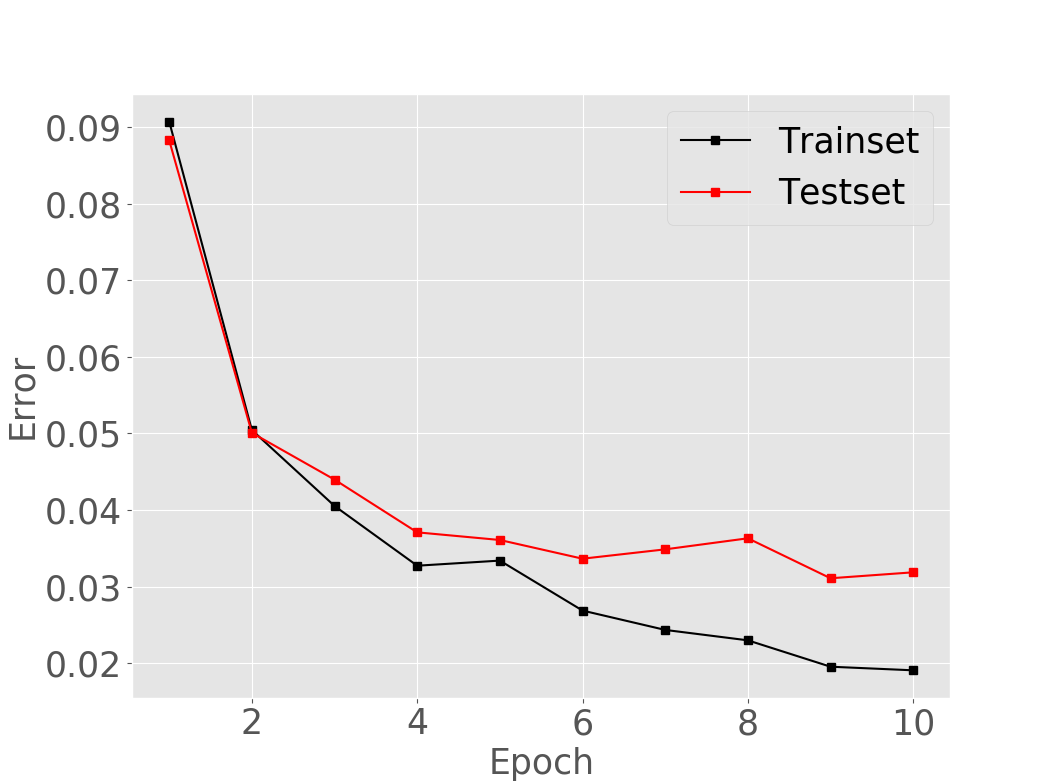
\includegraphics[width=.7\linewidth]{classerror}
	\captionof{figure}{Classification error on train/test set.}
\end{center}

Training trough minimization of the cross-entropy loss, which is equivalent to
\textit{perplexity}.  The standard metric for language
modeling\cite{gravesGenerating}.
\begin{figure}[htbp!]
\begin{tabular}{|l|l|c|}
\hline
Dataset & BPC & Perplexity \\
\hline
Harry Potter & 1.00 & 33 \\
LOTR & 1.02 & 35 \\
Random quotes & 1.10 & 45 \\
Shakespeare & 0.94 & 26\\
\hline
\end{tabular}
\end{figure}

\begin{itemize}\compresslist
    \item `` well , we ' ll do it with a wand , '' said hermione . `` really ?
      '' said harry , looking at each other .
    \item  what looked about this
      way , the black citadel , was far from the
          darkness , the ring was heard , but the sea big was big , and a great
          ring was in his battle .
    \item failure is a beginning of love and a family which comes from god .
    \item  '' that now my mind shall screens his music , '' '' and i to give
      thee my vulgar heaven , '' '' i am your brother .
\end{itemize}
\end{block}
\begin{block}{References}
\printbibliography
\end{block}
\end{column}
\separatorcolumn
\end{columns}
\end{frame}

\end{document}
